
\documentclass[11pt,a4paper]{article}
\usepackage{graphicx}
\usepackage{subfigure}


\title{MFEM: A Modular Finite Element Methods Library Summary}

\author{Muhammed Furkan Canga \\ 2168938}
\date{25 October 2023}
\begin{document}

\maketitle

\section{Abstract}

A detailed examination of MFEM, a flexible library of finite element techniques (FEM), may be found in the paper "MFEM: A modular finite element methods library," which was published in 2021 by Anderson et al. Complex partial differential equations can be solved with FEM, which is an essential tool in scientific and engineering simulations. MFEM provides a flexible and modular framework for this purpose. Because of MFEM's modular nature, customers can easily incorporate customized FEM applications into pre-existing software ecosystems and modify them to meet unique requirements.The paper emphasizes MFEM's potential in a range of computational applications by highlighting its significant characteristics, architecture, and capabilities. MFEM improves numerical simulation accuracy, facilitates high-performance parallel computing, and streamlines the implementation of FEM solvers. Because of its modular design, which enables users to assemble FEM applications like building bricks, it is an effective and adaptable tool for a variety of engineering and scientific projects.For researchers and practitioners seeking an effective and adaptable FEM library to expedite the creation of computational solutions and enhance the precision of their numerical simulations, this article is a priceless resource.


\section{Summary}
MFEM's modular architecture is its main strength. FEM applications frequently need complex customisation in order to fit into certain problem domains. By providing a framework within which users can combine FEM programs like building bricks, MFEM streamlines this procedure. The development of computational solutions can be streamlined by researchers and engineers by customizing simulations to meet their precise requirements thanks to this modularity.
\\
FEM is based on mathematical expressions, and MFEM provides a productive means of converting mathematical models into realistic simulations. Users may more easily express complex PDEs in code because to the library's architecture, which speeds up development and minimizes coding complexity. This feature makes FEM more approachable and frees researchers from the complexities of numerical implementation, allowing them to concentrate on their problem domain.
One of the most important expression which is heat conduction equation describes the distribution of temperature in a material over time. In one dimension, it is represented as:
\begin{equation}
\frac{\partial u}{\partial t} = \alpha \frac{\partial^2 u}{\partial x^2}
\end{equation}

Another significant equation is Poisson's equation which fundamental partial differential equation used to model various physical phenomena, including electrostatics. In two dimensions, it is expressed as:

\begin{equation}
\nabla^2 \phi = -\rho
\end{equation}

\\

High-performance parallel computing is essential in today's computing environment. PDEs are frequently solved on large grids or meshes in complex simulations, which calls for the distribution of computational tasks across a number of processors or computing nodes. Because it is made to take advantage of distributed computing environments and multi-core processors, MFEM excels in this area. Through the use of parallelism, MFEM enables researchers to quickly and effectively address computationally demanding problems.
\\

\begin{figure}[ht]
    \centering
    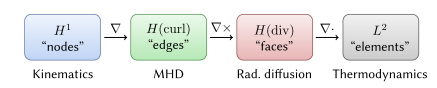
\includegraphics[width=0.7\textwidth]{hw1_fig1.png}
    \caption{Continuous de Rham complex in 3D and example physical fields that can be represented in the respective spaces}
    \label{fig1}
\end{figure}


A flexible framework that links solution spaces for different partial differential equations (PDEs) is the de Rham complex as shown in Figure \ref{fig1}. These solution spaces are discretized in MFEM using finite element spaces. Different finite element spaces, such as H1, ND, RT, or L2, are constructed depending on the type of PDE. Kinematic variables, electromagnetic fields, diffusion fluxes, and thermodynamic quantities can all be represented using these spaces. The de Rham complex is supported by MFEM at high orders and on various mesh types. GridFunctions in MFEM are piecewise-smooth functions on computational meshes and can be used for both linear alegbra operations and as discrete functions in particular FiniteElementSpaces.

\\

\begin{figure}
    \centering
    \subfigure[]{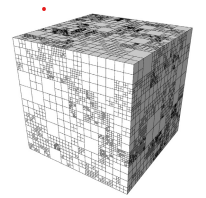
\includegraphics[width=0.24\textwidth]{hw1_fig2a.png}} 
    \subfigure[]{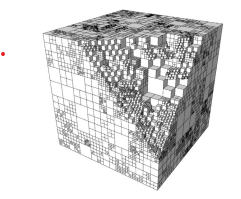
\includegraphics[width=0.24\textwidth]{hw1_fig2b.png}} 
    \subfigure[]{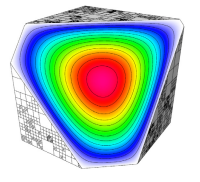
\includegraphics[width=0.24\textwidth]{Ekran görüntüsü 2023-10-26 213906.png}}
    
    \caption{(a) Randomly refined non-conforming mesh (b)  assemble of matrix A and vector b independently on each element (c) The interpolated solution}
    \label{fig:2}
\end{figure}

The application of parallel adaptive mesh refinement (AMR) to hexahedral and unstructured quadrilateral meshes in high-order applications is covered in this article as shown on Figure\ref{fig:2}. While these mesh types have benefits like flexibility in refinement and tensor product structure, they also come with drawbacks like hanging nodes. The emphasis is on non-conforming (irregular) meshes, where the degrees of freedom of adjacent elements may not be shared by them in whole, necessitating constraints. For parallel non-conforming meshes, MFEM presents its software abstractions and algorithms that support curved meshes and the full de Rham sequence of finite element spaces at arbitrary high order. 

\\
\begin{table}[h!]
\centering
\begin{tabular}{||c c c c||} 
 \hline
  & p=1 & p=2 & p=4\\ [0.5ex] 
 \hline\hline
 GPU OCCA-CUDA& 0.52 & 0.31 & 0.20 \\ 
 \hline
 Multicore OCCA-OMP& 3.34   &2.41 & 2.13 \\
 \hline
 CPU OCCA-CPU& 21.05   & 15.77 & 14.23 \\
 \hline
\end{tabular}
\caption{Performance Results of OCCA on different processors}
\label{table:1}
\end{table}
\\



The article talks about using the MFEM library to port existing codes to GPUs. In certain situations.Device object and turning on the partial assembly mode can make this procedure quite simple. In more complicated situations,  macros and memory management are more deeply understood, particularly when utilizing MFEM at a lower level. Several pre-defined integrators are not GPU-portable, and full assembly on GPUs is still unavailable, to name a couple of the limitations in GPU support. Further developments point to possible improvements in a variety of backends. OPPA  performances shown in the Table \ref{table:1} to understand the topic better.






\section{Conclusion}
For researchers and practitioners looking for a productive and adaptable FEM framework for their computational projects, the MFEM library is an invaluable resource. It has the ability to improve numerical simulation accuracy and expedite the development of computational solutions.

\bibliographystyle{plain}
\bibliography{bibll}
\cite{ANDERSON202142}

\end{document}


